% Final project report. Build: xelatex final_report.tex (twice). See report/README.md.
\documentclass[12pt,a4paper]{article}
\usepackage[a4paper,margin=2.5cm]{geometry}
\usepackage{fontspec}
\setmainfont{Times New Roman}
\setmonofont{Courier New}[Scale=0.833]
\usepackage{microtype}
\usepackage{graphicx}
\usepackage{booktabs}
\usepackage{array}
\usepackage{tikz}
\usetikzlibrary{positioning,arrows.meta,shapes.geometric}
\usepackage{titlesec}
\usepackage{caption}
\usepackage{fancyhdr}
\usepackage{xurl}
\usepackage[hidelinks]{hyperref}
\usepackage{ragged2e}

% Body: 12 pt, line spacing 1.15 (Word single = 1.15 em for TNR), 0 pt before / 6 pt after, no indent.
\newcommand{\bodyfont}{\fontsize{12}{15.87}\selectfont}
\newcommand{\tablefont}{\fontsize{10}{11.5}\selectfont}
\AtBeginDocument{\bodyfont}
\setlength{\parindent}{0pt}
\setlength{\parskip}{6pt}
\setlength{\emergencystretch}{3em}

% Headings: 14 pt bold / 12 pt bold, 12 pt before, 6 pt after, left-aligned.
\titleformat{\section}{\fontsize{14}{17}\selectfont\bfseries}{\thesection}{0.6em}{}
\titleformat{\subsection}{\fontsize{12}{15}\selectfont\bfseries}{\thesubsection}{0.6em}{}
\titlespacing*{\section}{0pt}{12pt}{6pt}
\titlespacing*{\subsection}{0pt}{12pt}{6pt}

% Captions: Times New Roman, 10 pt, single-spaced.
\captionsetup{font={small,stretch=1},labelfont=bf,skip=3pt,justification=centering}
\renewcommand{\small}{\fontsize{10}{11.5}\selectfont}

% Page numbers bottom right.
\pagestyle{fancy}
\fancyhf{}
\renewcommand{\headrulewidth}{0pt}
\fancyfoot[R]{\thepage}

\begin{document}
\raggedbottom
\begin{center}
{\fontsize{16}{19}\selectfont\bfseries AI-Assisted On-Call Queue: Budgeted Incident Detection for Cloud Microservices\par}
\vspace{6pt}
Aishah Mohamed Alyammahi
\end{center}

\vspace{-4pt}
\begin{center}\textbf{Abstract}\end{center}
\vspace{-8pt}
\begin{justify}
An on-call engineer can read only a few alerts a day, yet most real faults never write a log line, so rules that rank by log severity miss them. This project builds a queue that shows at most \textit{K} items a day, in the order a live system learns about them, and checks it on the public GAIA microservice benchmark. The queue combines rule-based metric detectors (memory jumps, slow leaks, monitoring gaps) with an optional cost-sensitive logistic-regression classifier for log alerts, and ships as a FastAPI service in one Docker container, in shadow mode by default. On 1{,}223 test faults at \textit{K}\,=\,20, the detector catches 72.6\% (best possible 84.9\%) against 68.9\% for a Prometheus rate rule and 0\% for log severity, and wins all 8 walk-forward weeks with 1.0 instead of 2.1 false items a day. The classifier adds no catches on GAIA, and the promotion gate keeps it out there; it helps on one of six RCAEval suites. The advantage over the rate rule is modest, and every GAIA fault is the same injected memory fault.
\end{justify}

\section{Motivation and objectives}
\textbf{Problem.} A platform of many small services raises thousands of alerts a day. The engineer on call can read about \textit{K}\,=\,20. Teams escalate by log severity and delete exact duplicates, or use fixed metric thresholds. On GAIA, 82\% of the injected faults write no log line and appear only as a jump in container memory, so log severity catches none of them at \textit{K}\,=\,20, and a fixed threshold either misses faults or floods the queue. GAIA injects about 22 faults a day, more than a 20-item budget on 34 of 55 days.

\textbf{Users and value.} The primary users are on-call engineers; secondary users are the operator who decides when the tool may page, and a team that wants to check the tool on its own data before trusting it. The value is a short, ordered, explained list that contains more real faults and fewer false items.

\textbf{Objectives.} O1: beat the rules a team already runs (log severity, static threshold, Prometheus rate rule) at \textit{K}\,=\,20. O2: decide in real time, using no later data. O3: engineer it for production (authentication, safe paging, versioned models with rollback, monitoring, Docker). O4: test it (at least 90\% of tests passing, coverage of at least 85\%, p95 latency of at most 1~s at 50 users). O5: let another team evaluate it on its own data without code.

\section{Architecture and implementation}
\begin{figure}[ht]
\centering
\begin{tikzpicture}[font=\fontsize{10}{11}\selectfont,
  box/.style={draw,rounded corners=2pt,align=center,minimum height=7mm,inner sep=3pt,fill=gray!8},
  ext/.style={draw,dashed,align=center,minimum height=7mm,inner sep=3pt},
  arr/.style={-{Stealth[length=2mm]},thick}]
\node[ext] (am) {Alertmanager\\(webhook)};
\node[ext,below=3mm of am] (pr) {Prometheus\\(memory)};
\node[box,right=9mm of am] (in) {Ingest\\validate, dedup};
\node[box,right=9mm of pr] (pull) {Metric fetch\\60 s steps};
\node[box,right=9mm of in] (det) {Detectors\\jump, leak, gap};
\node[box,right=9mm of pull] (clf) {Classifier\\log alerts};
\node[box,right=9mm of det,yshift=-7mm] (q) {Causal queue\\≤ \textit{K} a day};
\node[box,right=9mm of q] (pg) {Paging gate\\shadow / LIVE};
\node[ext,above=3mm of pg] (ch) {PagerDuty, Slack,\\Opsgenie};
\node[box,below=5mm of q] (st) {SQLite store, model registry,\\audit log, \texttt{/metrics}};
\draw[arr] (am)--(in); \draw[arr] (pr)--(pull);
\draw[arr] (in)--(det); \draw[arr] (pull)--(det); \draw[arr] (in)--(clf);
\draw[arr] (pull)--(clf);
\draw[arr] (det)--(q); \draw[arr] (clf)--(q); \draw[arr] (q)--(pg); \draw[arr] (pg)--(ch);
\draw[arr] (q)--(st);
\end{tikzpicture}
\caption{Architecture. Solid boxes run in one container; dashed boxes are external. Engineers' Real/Noise marks flow back through the store into the next model.}
\label{fig:arch}
\end{figure}

The code has two layers. \texttt{app/src/} is a library with no HTTP (detectors, causal queue, classifier, evaluation); \texttt{app/product/} is the web app, job pipeline, connectors, model registry and monitoring. The queue is first come, first served: a point is hot when it is 0.5~GB above the median of the previous 15 minutes, two hot points within two minutes confirm a jump, and a jump is shown at confirmation only if its rise passes a threshold learned on week 1 (0.62~GB). A 3-hour median catches slow leaks, a service silent for 10 minutes becomes a gap item, and log alerts may use at most a quarter of the slots. Nothing uses a later point, the end of a jump or its peak; \texttt{tests/test\_causality.py} checks this.

\textbf{Design decisions.} (1) Rules do the detection and learning is limited to a confirmation threshold and the log-alert classifier, because a rule can be read and audited. (2) Time split only: train on the first 7 days, test on the next 55, never shuffled. (3) Shadow mode is the default; live paging needs a password, a channel and the typed word LIVE. (4) A new classifier is promoted only if, on held-out data, the queue with it costs at least one missed fault less than the queue without log alerts and the queue it replaces (a miss costs 10, a false item 1); the operator can roll back. (5) Models are stored as skops archives, never pickle. (6) A single worker with SQLite, one container per team. Technologies: Python 3.12, scikit-learn, FastAPI, SQLite, Docker, uv with a hash-pinned lock, GitHub Actions.

\textbf{Changes from the proposal.} The proposal planned an alert classifier as the main result. Measurement showed that on GAIA the metric rules carry the result, so the classifier became an optional component behind the promotion gate. A code review also removed five uses of later-in-the-day information, which lowered the full queue from 70.2\% to 69.6\%. A real Prometheus integration test then found that a 121~s query step meant live jumps could never be confirmed; the fetch now uses 60~s steps.

\section{Testing, evaluation and results}
\textbf{Methods.} The suite has 431 tests: unit tests for detectors, queue and policy; API and pipeline integration tests with outbound calls mocked; AI-specific cases (malformed rows, one-class labels, a worse model not promoted); security tests (login lock, SSRF, CSRF); a Docker integration test against real Prometheus and Alertmanager; and a load test. CI runs lint, type checks, tests on two Python versions, a dependency audit and a Docker build. A script, \texttt{run\_validate.py}, checks every number in the long report against \texttt{app/results/}. Evaluation uses the 55 test days of GAIA MicroSS (1{,}223 faults), an 8-week walk-forward in which everything is re-learned from the past, and bootstrap intervals and sign tests.

\begin{table}[ht]
\centering\tablefont
\begin{tabular}{@{}lrrr@{}}
\toprule
System, \textit{K}\,=\,20 items a day & Caught & False/day & Precision\\
\midrule
Log severity + exact duplicates & 0.0\% & 0.8 & 0\%\\
Static rule (week-1 99th percentile) & 57.2\% & 3.0 & 81\%\\
Prometheus rate rule & 68.9\% & 2.1 & 88\%\\
Detector alone (jump + learned threshold) & \textbf{72.6\%} & \textbf{1.0} & 94\%\\
Full queue with classifier (refused on GAIA) & 69.6\% & 1.8 & 90\%\\
Shipped queue (log alerts by severity) & 71.0\% & 1.4 & 92\%\\
\bottomrule
\end{tabular}
\caption{Faults caught of 1{,}223 (best possible at \textit{K}\,=\,20: 84.9\%).}
\label{tab:main}
\end{table}

\textbf{Results.} Table~\ref{tab:main} shows the detector beats the rate rule in 8 of 8 weeks (sign test \textit{p}\,=\,0.0039) with fewer false items. The full queue does not beat it week by week (4 wins, 3 losses, 1 tie), so the first claim is the detector. Median time to confirm is 0.72 minutes. Only 2\% of misses are the detector's fault: 45\% fall in a monitoring outage and 53\% lose to the budget. The classifier ablation is the main negative result: with classifier-chosen log alerts the queue catches 69.6\%, with severity-chosen alerts 71.0\%, with none 71.2\%. On RCAEval RE2 Train Ticket the classifier adds 13.3 points over no log alerts (95\% interval +4.4 to +24.4), but that gate decision was made on the same 45 cases that are scored, and on the other five suites it adds at most one case. A robustness replay shows the learned threshold over-fits 1~GB faults: it rejects every 0.5~GB fault, so it is off unless trained on a team's own incidents. Under load the app serves 50 users with p95 0.32~s and 0\% errors, and one GAIA month scores in 54.9~s with 505~MB peak memory.

\textbf{Beyond GAIA.} The same engine, tuned on the first half of each series, was run on NAB (five cloud, traffic and machine datasets), SMD (28 servers with CPU, memory, disk and network faults) and RCAEval (three microservice applications). On SMD it catches 55.1\% of 196 incidents at 20 items a day per machine against a 12.4\% chance line, but with low precision (11 false items a day). On NAB it is clearly above chance on traffic and machine data and no better than chance on Twitter volume. On RCAEval RE1 memory faults the jump rule overlaps 61--100\% of faults, but the budgeted queue catches 0 of 13 on every application. These failures are reported in the repository, not hidden: they show the 0.5~GB jump size and the learned threshold must be set for each team's own services.

\textbf{Against the criteria.} Tests: 421 pass, 10 skip (nine need torch, xgboost or CUDA; one needs Docker), 0 fail; coverage 86\%; p95 0.32~s. O1 is met for the detector and tied for the full queue; O5 is met, with NAB, SMD and RCAEval results including failures. No live pilot with a real team was run.

\section{Deliverables, setup and use}
\textbf{Repository.} \url{https://github.com/amamsy90/alert-fatigue-reduction}, version 1.1.0, submitted commit \texttt{COMMIT\_HASH}. The README lists the team, structure, prerequisites, exact commands, the tested system and the data sources. No paid API is needed and the system calls no external AI service.

\textbf{Setup and use.} From \texttt{app/}: \texttt{docker compose up -d} serves the app at \texttt{127.0.0.1:8080} in shadow mode; for development, \texttt{uv sync --group dev}, \texttt{uv run pytest -q} and \texttt{uv run python run\_validate.py} reproduce the test results and check the reported numbers against the committed result files. Re-running the experiments needs the GAIA data (about 1.8~GB, fetched by \texttt{tools/fetch\_gaia.py} with SHA-256 checks). Workflow: Alertmanager posts alerts, a job pulls memory from Prometheus and builds the day's queue with a reason for each item, the engineer marks items Real or Noise, and the marks train the next model. The \texttt{/evaluate} page runs the same engine on a team's own CSV files.

\section{Conclusion}
The project delivers a tested, deployable, causal on-call queue. Its measured contribution is a metric detector that catches 72.6\% of GAIA faults at 20 items a day with 1.0 false item, against 68.9\% and 2.1 for a Prometheus rate rule. Its main findings are negative or limited: the log-alert classifier earns its slots only where faults write logs, the full queue ties the rate rule, and all GAIA faults are one injected shape. The next step is a shadow-mode pilot with a real team.

\textbf{Limitations and honest use of tools.} The work is a solo project. AI coding assistants were used for code review, refactoring, test writing and drafting documentation (see \texttt{AGENTS.md} and the pull-request history); the running system uses no generative AI. Design decisions, the evaluation method and the claims made here are the author's responsibility. The timings come from one Windows laptop and are not a benchmark of other hardware.

\newpage
\appendix
\section{Walk-forward results}
\begin{table}[ht]
\centering\tablefont
\begin{tabular}{@{}lrrrrr@{}}
\toprule
Test week (2021) & Faults & With metrics & Rate rule & Detector & Full queue\\
\midrule
8--15 Jul & 161 & 100\% & 77.6\% & 84.5\% & 82.0\%\\
15--22 Jul & 134 & 91\% & 73.9\% & 81.3\% & 74.6\%\\
22--29 Jul & 162 & 94\% & 72.2\% & 77.2\% & 71.0\%\\
29 Jul--5 Aug & 163 & 82\% & 67.5\% & 69.3\% & 67.5\%\\
5--12 Aug & 162 & 84\% & 69.1\% & 71.6\% & 71.0\%\\
12--19 Aug & 139 & 92\% & 75.5\% & 79.1\% & 74.1\%\\
19--26 Aug & 173 & 61\% & 51.4\% & 52.0\% & 50.9\%\\
26--31 Aug & 129 & 91\% & 78.3\% & 83.7\% & 79.1\%\\
\midrule
Mean & & & 70.7\% & 74.8\% & 71.3\%\\
\bottomrule
\end{tabular}
\caption{Walk-forward at \textit{K}\,=\,20. The 19--26 Aug fold has a 2.5-day metric outage.}
\end{table}

\section{Classifier on other data}
\begin{table}[ht]
\centering\tablefont
\begin{tabular}{@{}llrrrl@{}}
\toprule
Suite & Application & Cases & No log alerts & Classifier & Gate\\
\midrule
RE2 & Online Boutique & 45 & 44.4\% & 46.7\% & refused\\
RE2 & Sock Shop & 45 & 84.4\% & 86.7\% & refused\\
RE2 & Train Ticket & 45 & 60.0\% & 73.3\% & promoted\\
RE3 & Online Boutique & 15 & 100\% & 100\% & refused\\
RE3 & Sock Shop & 15 & 93.3\% & 93.3\% & refused\\
RE3 & Train Ticket & 15 & 100\% & 100\% & refused\\
\bottomrule
\end{tabular}
\caption{RCAEval, share of test faults caught at \textit{K}\,=\,10. The gate ran on the same cases that are scored.}
\end{table}

\section{Figures}
\begin{figure}[ht]
\centering
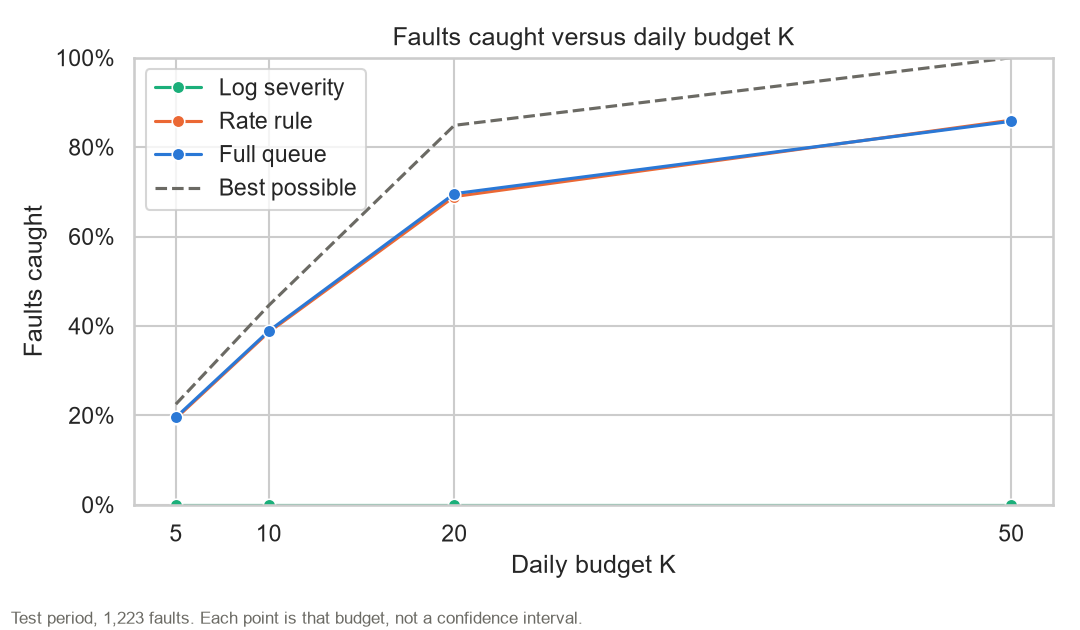
\includegraphics[width=0.8\textwidth]{../figures/detection_vs_k.png}
\caption{Faults caught versus daily budget \textit{K} on GAIA.}
\end{figure}
\begin{figure}[ht]
\centering
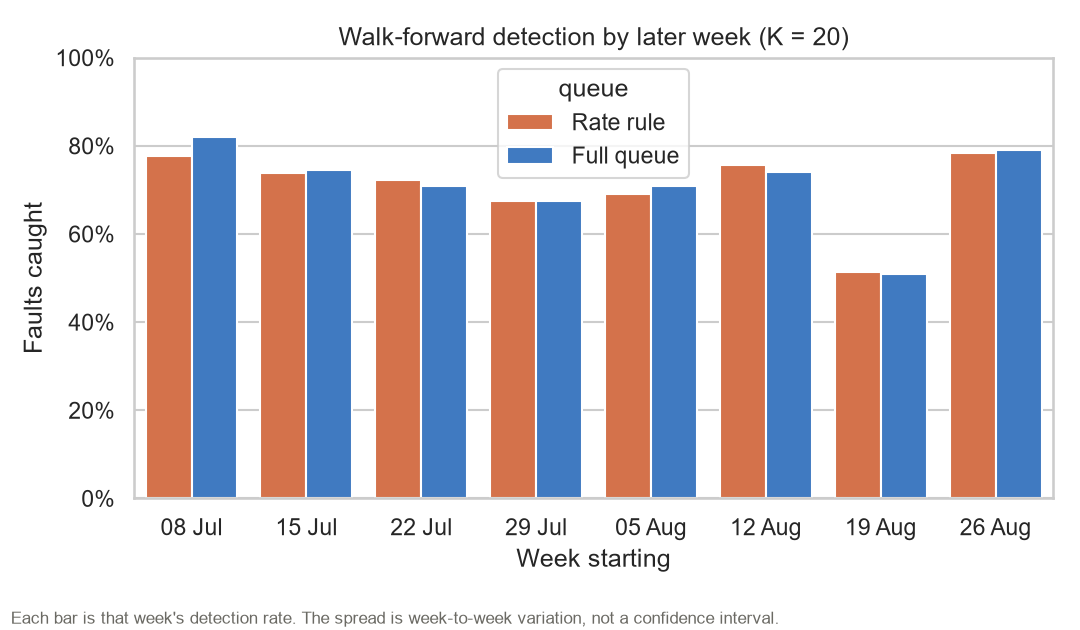
\includegraphics[width=0.8\textwidth]{../figures/walkforward.png}
\caption{Walk-forward detection by later week.}
\end{figure}
\end{document}
